В данной главе описаны возможные технологии распределённых реестров. Под
технологиями понимаются алгоритмы, протоколы, а так же общая структура реестра.
Распределённые реестры делятся на открытые (Public), закрытые (Private),
эксклюзивные (Permissioned), и инклюзивные (Permissionless).
По структуре реализации распределённые реестры делятся на 2 вида: блокчейны и
направленные ациклические графы (DAGs). Алгоритмы, представленные во всех типах
являются неотъемлимой их частью. Это алгоритмы хэширования, электронных
подписей, генерации случайных чисел. Специфические для конкретных реестров
алгоритмы, обеспечивающие должный уровень безопасности/анонимности, например
Ring signatures, Coinjoin, Coinshuffle, stealth addresses, MimbleWimble, etc.
будут рассмотрены в Главе 2. Помимо алгоритмов, будут рассмотрены и различные
протоколы консенсуса, (общей сложностью более 20 штук), обеспечивающие защиту и
надёжность транзакций в открытых блокчейнах.

\subsection{Виды распределённых реестров}\label{kinds_reestrs}
Для разделения реестров на группы по признакам открытости и закрытости
существует несколько подходов.
\begin{itemize}
    \item Первый --- канадский, основанный на публикации статьи
        \cite{VitalikButerin2015} создателя криптовалюты Ethereum Виталика
        Бутерина. Автор разделяет 3 типа реестров:
          \begin{enumerate}
              \item Публичный (Public), где каждый может принять участие в
                  создании блоков, которое никем не контролируются и
                  выполняется в свободном порядке;
              \item Приватный (Fully Private), где все транзакции отслеживаются
                  и контроллируются централизованной сущностью;
              \item Реестры консорциума (Consortium), где только избранные узлы
                  цепи контроллируют создание новых блоков.
          \end{enumerate}
     \item Второй --- британский. Определения Сэра Марка Уолпорта, главного
         научного советника Соединённого Королевства, в докладе о
         распределённых реестрах \cite{DeLeon2018}, совпадают по своей сути с определениями
         Бутерина, но отличаются названиями:
         \begin{enumerate}
                 \item Unpermissioned public;
                 \item Permissioned private;
                 \item Permissioned public.
         \end{enumerate}
     \item Третий --- российский. Часто, для избежания недопониманий и
         сложностей в определении, мировые эксперты используют понятия
         Публичный (Открытый) и Приватный (Закрытый) реестры. Российские
         эксперты не исключение. В своём докладе \cite{2016}, Ольга Скоробогатова,
         заместитель председателя ЦБ РФ, разделяет реестры именно таким
         образом. Данное разделение будет использоваться в настоящей работе:
         \begin{enumerate}
             \item Публичный (Открытый, Public, Open). В открытых реестрах нет
                 контроллирующей стороны, как это реализовано в закрытых
                 реестрах, все транзакции происходят в свободном порядке, а для
                 подтверждения легитимности транзакции используются специальные
                 протоколы консенсуса (\ref{consensus_protocols})
             \item Приватный (Закрытый, Private, Closed).  Не смотря на то, что
                 сама рассматриваемая технология является распределённой,
                 элементы централизованности присутствуют в таких вариантах,
                 как закрытые (\ref{kinds_reestrs}) реестры. Закрытым реестр
                 может являться благодаря первичному блоку (в случае
                 блокчейна), который будет использоваться. Любой узел может
                 присоединиться к приватному реестру, если он знает адрес
                 начального узла для синхронизации и идентификатор сети. Этот
                 узел может выполнять любые действия в закрытом реестре:
                 майнить, совершать транзакции, заключать контракты, и т.д.\\

                 Такие реестры зачастую используюся фирмами, банками и т.д. для
                 организации внутренних операций обмена и регистрирования.
         \end{enumerate}
\end{itemize}

\subsection{Структура реестров}
По своей внутренней структуре представления распределённые реестры делятся на
блокчейны (\ref{struct_block}) и направленные ациклические графы
(\ref{struct_dags}). На рисунке \ref{graph_reester} изображены виды современных
распределённых реестров.

\begin{figure}[h]
    \Tree [.DL [.DAG ] [.Blockchain ] [.Hybrids\ \&\ Others ]]
    \caption{Виды распределённых реестров}\label{graph_reester}
\end{figure}

\subsubsection{Блокчейны}\label{struct_block}
Блокчейны --- наиболее распространённые сегодня виды реестров. Набор транзакций
(операций) собирается в один блок. Проходит определенное время и этот блок
добавляется в общую цепочку. Для подтверждения транзакции существует множество
протоколов консенсуса --- стандартов, исходя из которых можно говорить, что
создание и добавление данного блока имеет место быть. Подтверждение легальности
добавления блоков в других представлениях распределённых реестров происходит с
приминением других алгоритмов и протоколов, поэтому далее для протоколов
консенсуса будет использоваться слово ``блокчейн'' вместо ``реестр'' для
исключения возможности двоякой интерпретации (на самомм деле, в некоторых
реализациях DAG \cite{Popov2018} может применяться протокол консенсуса
\ref{pow} для защиты от спама). Блокчейны завоевали стратегические позиции на
площадке распределённых реестров и ``прошли проверку временем'', но появляются
новые технологии, такие как DAG и другие, призванные решить некоторые
недостатки сетей блокчейн, речь о которых пойдёт позже.

\subsubsection{Направленные ациклические графы (DAGs)}\label{struct_dags}
В DAG все новые записи добавляются в общую цепочку (корректнее --- граф)
асинхронно. История записи операций выглядит как направленный ациклический граф
(wiki). DAG топологически отсортирован так, что каждое ребро направлено от
более раннего ребра к более позднему.

\subsubsection{Плюсы и минусы DAG}
Рассмотрим некоторые преимущества и недостатки DAG по отношению к блокчейнам.\\
Плюсы:
\begin{itemize}
    \item Масштабируемость
    \item Мнгновенные транзакции
    \item Отсутствие либо чрезмерно малые (не заметные) комиссии за переводы
\end{itemize}
Эти плюсы открывают дорогу для огромного количества микротранзакций, делая
систему пригодной, для, например, интернета вещей.\\
Минусы:
\begin{itemize}
    \item Возможные в будущем проблемы с масштабируемостью
    \item Нет подтверждённой учёными информации о защите от взлома основанных на DAG систем
\end{itemize}

\subsection{Алгоритмы}
Рассмотрим некоторые криптографические алгоритмы, которые используются в описанных системах.
\subsubsection{SHA-256}
Алгоритм хэширования SHA-256, работая с данными, разбитыми на кусочки по 512
бит (64 байт), смешивает их криптографически и выдаёт 256-битный (32 байта) хэш
--- уникальную (почти) сигнатуру входного текста.
\subsubsection{ECDSA}
Алгоритм цифровой подписи ECDSA (Elliptic Curve Digital Signature Algorithm)
--- криптографический алгоритм, используемый в целях гарантировать, что узлы
сети могут быть использованы только их законными владельцами. Использует
концепты публичного и приватного ключа. В алгоритме публичный ключ-это
уравнение для эллиптической кривой и точка, лежащая на этой кривой. Приватный
ключ-это число.

\begin{figure}[h]
    \centering
    \begin{tikzpicture}
        \begin{axis}[
            xmin=-2,
            xmax=4,
            ymin=-7,
            ymax=7,
            xlabel={$x$},
            ylabel={$y$},
            scale only axis,
            axis lines=middle,
            % set the minimum value to the minimum x value
            % which in this case is $-\sqrt[3]{7}$
            domain=-1.912931:3,      % <-- works for pdfLaTeX and LuaLaTeX
            % domain=-1.91293118:3,   % <-- would also work for LuaLaTeX
            samples=200,
            smooth,
            % to avoid that the "plot node" is clipped (partially)
            clip=false,
            % use same unit vectors on the axis
            axis equal image=true,
        ]
            \addplot [blue] {sqrt(x^3+7)}
                node[right] {$y^2=x^3+7$};
            \addplot [blue] {-sqrt(x^3+7)};
        \end{axis}
    \end{tikzpicture}
    \caption{Эллиптическая кривая}\label{elliptic_curve}
\end{figure}


\subsection{Особые алгоритмы}
Помимо стандартных криптографических алгоритмов шифрования, генерации
электронной подписи и случайных чисел, в распределённых реестрах повсеместно
используются алгоритмы, обеспечивающие сокрытие персональных данных и адресов
отправителей и получателей, алгоритмы по защите и обфусцированию данных,
отправляющихся по небезопасным каналам связи.
\subsubsection{Ring Signatures}
Представлен впервые в Декабре 2012 \cite{VanSaberhagen2012} Cryptonote. Вторая версия документа
Cryptonote v2 --- Октябрь 2013 \cite{VanSaberhagen2013}.
Такая криптовалюта как Monero использует технологию кольцевой
подписи для защиты конфиденциальности пользователя при проведении транзакций.
Кольцевые подписи скрывают информацию об отправителе, заставляя отправителя
подписывать транзакцию с помощью подписи, которая может принадлежать нескольким
пользователям. Это делает транзакцию неотслеживаемой.\\
Интересно рассмотреть вариацию данного алгоритма RingCT, которая будет
рассмотрена далее (\ref{ringct})
\subsubsection{Stealth Addressess}
Представлены в том же документе. Stealth addresses позволяют получателю
предоставлять для получения один адрес, который генерирует другой публичный
адрес для средств, которые будут получены каждый раз при отправке на него. Это
делает транзакцию так же, неотслеживаемой.\\

Поскольку алгоритмы определены в одной работе и имеют схожие цели, можно,
объединив их, назвать основные плюсы и минусы:\\
\textbf{Плюсы}
\begin{itemize}
    \item Обеспечивает конфиденциальность отправителя и получателя
    \item Конфиденциальность может гарантироваться по умолчанию
    \item Проверенная технология
    \item Не требует каких-либо третьих сторон
\end{itemize}
\textbf{Минусы}
\begin{itemize}
    \item Конфиденциальность не очень эффективна, имея недостаточный объем
          хранилища
    \item Не скрывает информацию о самой транзакции (если алгоритм
          используется сам по себе, не объединяясь с другими)
\end{itemize}

\subsubsection{Coinjoin, coinshuffle}
Разработчик Биткоина Грегори Максвелл предложил набор решений для обеспечения
конфиденциальности в распределённых реестрах и криптовалютах, первым из которых
являлся CoinJoin. \cite{Maurera}. CoinJoin (иногда называемый CoinSwap)
позволяет нескольким пользователям объединять свои транзакции в одну
транзакцию, получая входы от нескольких пользователей, а затем отправляя свои
выходы нескольким пользователям, независимо от того, от кого в группе пришли
входы. Таким образом, получатель получит назначенную сумму, но будет
невозможным отследить транзакцию вплоть до отправителя.\\
\textbf{Плюсы}
\begin{itemize}
    \item Обеспечивает конфиденциальность отправителя и получателя
    \item Простота реализации на любой криптовалюте
    \item Легковесная реализация в коде
    \item Проверенная технология
\end{itemize}
\textbf{Минусы}
\begin{itemize}
    \item Суммы смешанных транзакций могут быть выссчитаны
\end{itemize}

\subsubsection{Sigma Protocol}
Sigma Protocol --- активно исследуется командой Zcoin с 2018 года для замены
протокола Zerocoin zk-Snarks (zero knowledge succinct non-interactive arguments of
knowledge) для того, чтобы не требовалась доверенная
преднастройка. \cite{Groth2015}. Существует возможная замена zk-Snarks,
называемая zk-Starks, другая форма доказательства нулевого знания, которая
может сделать доверенную преднастройку ненужной для монет с нулевым знанием.

\subsubsection{Zerocash}
В мае 2014 года был создан нынешний преемник протокола Zerocoin, Zerocash. Он
улучшил концепцию Zerocoin, воспользовавшись уже известным zk-Snarks. В отличие
от Zerocoin, который скрывал происхождение оригинальных монет и историю
платежей, Zerocash был быстрее, с меньшими размерами транзакций и скрывает
информацию о транзакции отправителя, получателя и суммы транзакций.
Zcash-первая криптовалюта, реализовавшая протокол Zerocash в 2016 году.
\cite{ZerocoinElectricCoinCompany2016}

\subsubsection{CT, RingCT}\label{ringct}
Confidential Transactions были представлены обществу в 2015 году \cite{Maxwell}
Было предложено скрыть сумму транзакции и тип передаваемых данных (например,
депозиты, валюты, акции), чтобы только отправитель и получатель знали о сумме
(до тех пор, пока они не решат сделать сумму общедоступной). В алгоритме
используется гомоморфное шифрование для шифрования входов и выходов.\\

Затем появились Ring Confidential Transactions \cite{Noether2016}.  RingCT
сочетает использование кольцевых подписей для сокрытия информации об
отправителе с использованием конфиденциальных транзакций (которые также
используют кольцевые подписи) для сокрытия сумм. В работе описан новый тип
кольцевой подписи --- A Multi-layered Linkable Spontaneous Anonymous Group,
многослойная связанная спонтанная анонимная групповая подпись, которая
``позволяет скрывать суммы, происхождение и назначение транзакций, с разумной
эффективностью и качественной проверкой, с возможностью не-доверительной
генерации монет''.

\subsubsection{MimbleWimble}
Mimblewimble \cite{Poelstra2016} использует концепцию Confidential Transactions
для скрытия сумм, а для доказательства права на собственность, смотрит на
закрытые ключи и информацию о транзакциях, а не на адреса, так же, связывает
транзакции вместе, а не рассматривает их отдельно на блокчейне. Grin-это
криптовалюта, находится в состоянии разработки и применяет Mimblewimble.

\subsubsection{Zexe}
В Октябре 2018 Zexe был представлен новый криптографичекий концепт ---
``децентрализованные частные вычисления'' (decentralized private computation)
\cite{Bowe2019}. Он позволяет пользователям распределённых реестров ``выполнять
автономно вычисления у себя на машинах, результатами которых будут настоящие
транзакции'', а также сохраняет суммы транзакций скрытыми и позволяет проверять
транзакции в любое время независимо от вычислений, выполняемых в интернете.

\subsection{Протоколы консенсуса}\label{consensus_protocols}
Протокол консенсуса --- стандарт, описывающий правила создания блоков в
открытых распределённых реестрах. В работе рассмотрены все протоколы
консенсуса, используемые в распространённых на сегодняшний день распределённых
реестрах.
\subsubsection{Proof of Work (PoW)}\label{pow}
Впервые концепция Proof of Work была описана в 1993 году в работе ``Pricing via
Processing, Or, Combatting Junk Mail, Advances in Cryptology''
\cite{Dwork2007}.

Идея авторов заключалась в следующем: чтобы получить доступ к общему ресурсу,
пользователь должен вычислить некоторую достаточно сложную функцию, и так
защитить ресурс от злоупотребления.  В 1997 году Адам Бэк запустил проект
Hashcash, посвященный той же защите от спама. Задача формулировалась следующим
образом: «Найти такое значение x, что хеш SHA(x) содержал бы N старших нулевых
бит».

Алгоритм PoW используется в открытых реестрах
для создания новых блоков. Алгоритм хорошо проявляет себя для доказательства
легитимности транзакции, выполняя которое, майнеры вознаграждаются процентом,
соответствующим вычислительной сложности всей сети. Зарекомендовавшее себя
средство, оно не является выгодным с точки зрения расхода природных ресурсов,
поскольку объём энергозатрат для выполнения вычислений, необходимых на
добавление одного блока, сопоставим с объемом энергии, потребляемым двумя
средними американскими домами: `` Bitcoin transaction uses roughly enough
electricity to power 1.57 American households for a day.'' --- \cite{amhouses}

\subsubsection{Proof of Stake (PoS)}
Алгоритм доказательства доли владения --- основной конкурент предыдущего
алгоритма. Вероятность формирования участником очередного блока в реестре
пропорциональна доле, которую составляют принадлежащие этому участнику
расчётные единицы данного реестра (напр., кол-во единиц криптовалюты) от их
общего количества. Поскольку для принятия решения о том, кто будет являться
создателем нового блока, нет необходимости в большом объёме вычислений, как в
PoW, зачастую является выбором, когда экологический фактор поставлен на одно из
главных мест.

\subsubsection{Delegated Proof-of-Stake (DPoS)}
Delegated PoS применяет PoS с расширенным функционалом. Поэтому остается
быстрым (и даже ещё быстрее), не требует больших вычислительных мощностей по
сравнению с алгоритмом Proof of Work (PoW). Суть DPoS состоит в том, что узлы
сети методом голосования выбирают узел, который будет генерировать блоки. В
этом случае работает правило: чем большим количеством монет обладает узлы, тем
больший вес имеет ее голос. Правила начисления вознаграждения также
определяются также участниками сети. В некоторых сообществах вознаграждение
начисляется не только узлы, которой делегировали право генерировать блоки, но и
остальным участникам. Первая криптовалюта, в которой был применен алгоритм DPoS
--- Bitshares. Также он применяется в следующих проектах: EOS, Steemit.

\subsubsection{Proof-of-Authority (PoA)}
Алгоритм доказательства полномочий --- это ещё один алгоритм консенсура, в
котором транзакции проверяются специальными учетными записями (валидаторами)
системы. То есть майнить могут только валидаторы. Как пример использования
можно привести систему Kovan Testnet \cite{Etherium2018}.

\subsubsection{Byzantine Fault Tolerance (BFT)}
Лэсли Лэмпорт в 1982 году \cite{Lamport2002} со своими соавторами представили
общественности задачку о Византийских генералах, позже использованную для
создания алгоритма консенсуса BFT.

В BFT, как и в PoA существуют валидаторы, и только им позволено совершать
быстрые транзакции, управлять каждым состоянием сети и обмениваться сообщениями
друг с другом, чтобы получить правильную запись транзакции и обеспечить
честность. Данный алгоритм реализуется компанией Ripple, где валидаторы
выбираются предварительно. Любой может быть валидатором --- доверие
устанавливается сообществом. В отличие от блокчейнов, основанных на PoW,
блокчейны BFT не подвергаются нападению, если только сами пользователи сети не
координируют атаку. BFT считается выгодным алгоритмом, поскольку он
масштабируем и охватывает транзакции с низкой стоимостью, но, как и DPoS,
внедряет компонент централизации.

\subsection{Выводы по главе}
В данной главе были рассмотрены основные и наиболее распространённые алгоритмы
и протоколы в распределённых реестрах сегодняшнего дня. Поскольку в рассчёт
брались только популярные, этого должно хватить для понимания общей картины
текущего криптопротокола, но работа нацелена на глубокое изучение. На рис.
\ref{2014protocol} \cite{TimSwanson2014} приведена структура используемых
алгоритмов и протоколов в распределённых реестрах на 2014 год. На сегодняшней
день многое поменялось и добавились новые алгоритмы и протоколы, появились даже
новые распределённые реестры, не основанные на блокчейне. На
рис.\ref{myprotocol} приведена классификация обновлённая, на Q2 2019 года. На
ней очевидны изменения в количественную сторону.

\newpage
\begin{figure}[h!]
    \centering
    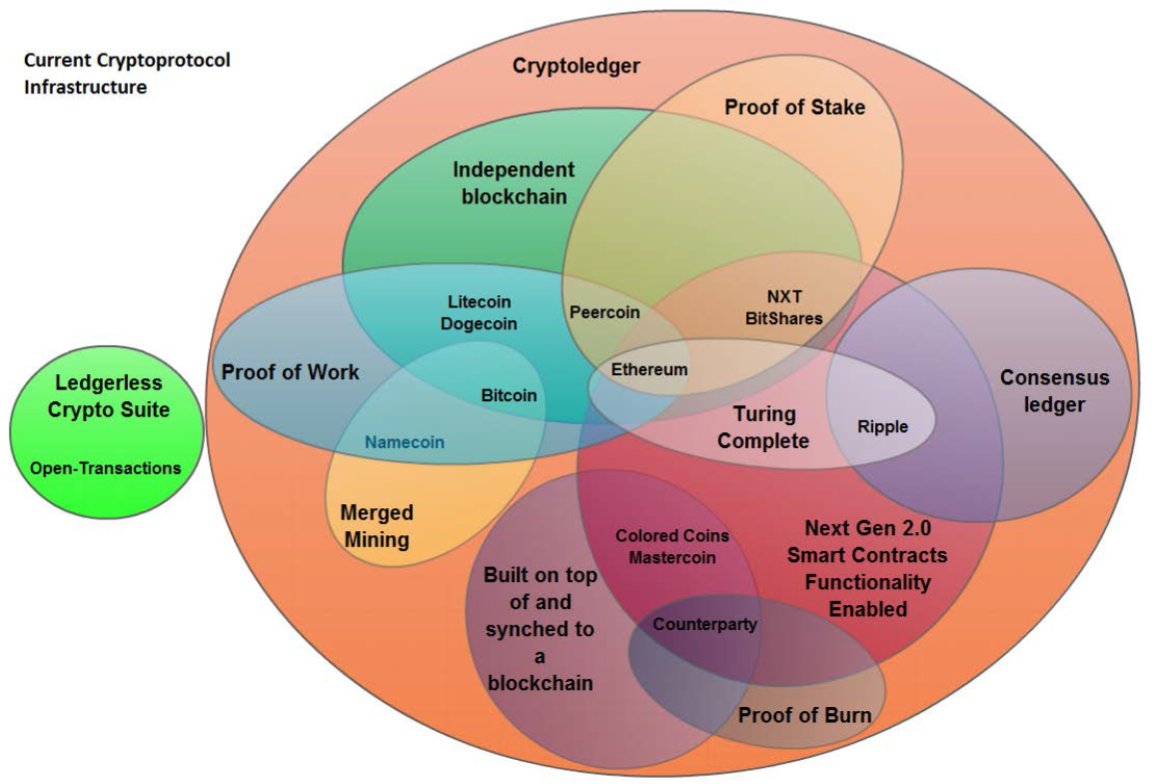
\includegraphics[width=0.8\textwidth]{./images/current_protocols}
    \caption{Классификация на 2014 год}\label{2014protocol}
\end{figure}


\begin{figure}[h!]
    \centering
    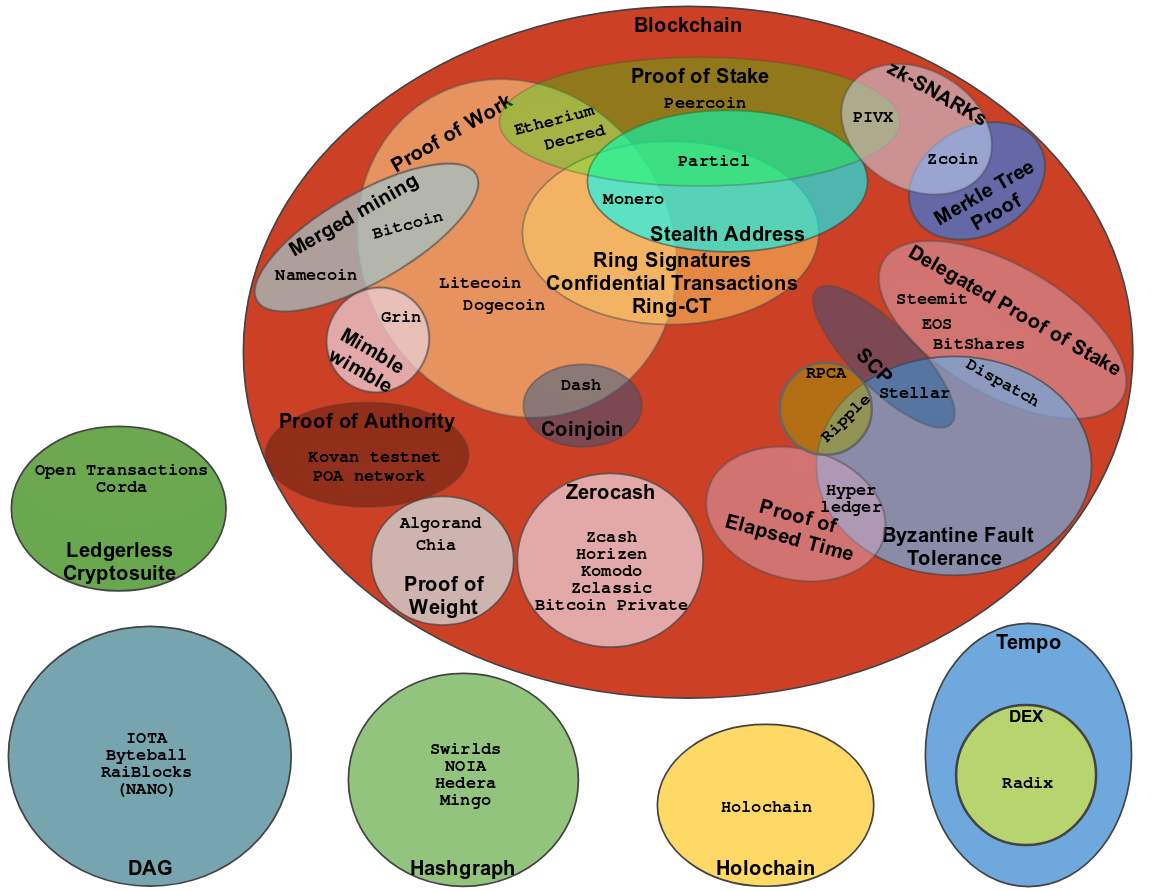
\includegraphics[width=.8\textwidth]{./images/myprotocol}
    \caption{Классификация на 2019 год}\label{myprotocol}
\end{figure}
